% Unofficial University of Cambridge Poster Template
% https://github.com/andiac/gemini-cam
% a fork of https://github.com/anishathalye/gemini
% also refer to https://github.com/k4rtik/uchicago-poster

\documentclass[final]{beamer}

% ====================
% Packages
% ====================

\usepackage[T1]{fontenc}
\usepackage{lmodern}
\usepackage[size=custom,width=120,height=72,scale=1.0]{beamerposter}
\usetheme{gemini}
\usecolortheme{cam}
\usepackage{graphicx}
\usepackage{booktabs}
\usepackage[numbers]{natbib}
\usepackage{tikz}
\usepackage{pgfplots}
\pgfplotsset{compat=1.14}
\usepackage{anyfontsize}

% ====================
% Lengths
% ====================

% If you have N columns, choose \sepwidth and \colwidth such that
% (N+1)*\sepwidth + N*\colwidth = \paperwidth
\newlength{\sepwidth}
\newlength{\colwidth}
\setlength{\sepwidth}{0.025\paperwidth}
\setlength{\colwidth}{0.3\paperwidth}

\newcommand{\separatorcolumn}{\begin{column}{\sepwidth}\end{column}}

% ====================
% Title
% ====================

\title{Dinkelbach Algorithm for SBPO Challenge 2025}

\author{Santiago Cifuentes \inst{1} \and Ignacio Oromendia \inst{1} \and Luciana Skakovsky \inst{1}}

\institute[shortinst]{\inst{1} FCEN - Universidad de Buenos Aires }

% ====================
% Footer (optional)
% ====================

\footercontent{
  \href{https://www.example.com}{https://www.example.com} \hfill
  SBPO 2025 \hfill
  \href{mailto:alyssa.p.hacker@example.com}{alyssa.p.hacker@example.com}}
% (can be left out to remove footer)

% ====================
% Logo (optional)
% ====================

% use this to include logos on the left and/or right side of the header:
% \logoright{\includegraphics[height=7cm]{logo1.pdf}}
% \logoleft{\includegraphics[height=7cm]{logo1.pdf}}

% ====================
% Body
% ====================

\begin{document}

% Refer to https://github.com/k4rtik/uchicago-poster
% logo: https://www.cam.ac.uk/brand-resources/about-the-logo/logo-downloads
\addtobeamertemplate{headline}{}
{
    \begin{tikzpicture}[remember picture,overlay]
      \node [anchor=north west, inner sep=3cm] at ([xshift=0.0cm,yshift=1.0cm]current page.north west)
      {
\includegraphics[height=4.5cm]{logos/cambridge-reversed-color-logo.eps}}; 
    \end{tikzpicture}
}

\begin{frame}[t]
\begin{columns}[t]
\separatorcolumn

\begin{column}{\colwidth}

  \begin{block}{The Problem}

    In warehouse operations, picking each order individually is inefficient. Instead, we group compatible orders into \textbf{waves} so that their items can be collected together through shorter and more efficient routes. The goal is to decide which orders should form the next wave to maximize \textbf{picking productivity} — that is, to collect as many products as possible while visiting as few aisles as needed.

Let $O$ be the set of pending orders, $I_o$ the items requested in order $o\in O$, 
$A$ the set of aisles, and $A_i\subseteq A$ the aisles containing item $i$. 
Each order $o$ requests $u_{oi}$ units of item $i$, and each aisle $a$ holds $u_{ai}$ units. 
Wave size is bounded by $LB, UB$ lower and upper bounds on the total number of items in the wave.


We want to select:
\[
O' \subseteq O \quad \text{(orders in the wave)}, \qquad
A' \subseteq A \quad \text{(aisles to visit)}
\]
so as to maximize the ratio between collected units and visited aisles:

\[
\max_{O',A'} \; \frac{\displaystyle\sum_{o \in O'} \sum_{i \in I_o} u_{oi}}{|A'|}
\]

subject to:
\begin{align}
    & LB \le \sum_{o \in O'} \sum_{i \in I_o} u_{oi} \le UB \tag{1}\\[3pt]
    &\sum_{o \in O'} u_{oi} \le \sum_{a \in A'} u_{ai}, \quad \forall i \in I_o, \; o \in O' \tag{2}
\end{align}

A pair $(O',A')$ satisfying (1)--(2) defines a feasible wave, and the optimal wave maximizes the productivity ratio above.
  \end{block}

\begin{block}{An Exact Parametric Approach}

We apply a parametric algorithm based on Dinkelbach’s method to solve the fractional objective. 
The problem is reformulated as finding the root of a convex function:
\[
\phi(\lambda) = \max_{x \in X} \{ f(x) - \lambda g(x) \},
\]
where $f(x)$ and $g(x)$ are linear. Each evaluation of $\phi(\lambda)$ is obtained by solving a linear program (LP). 
In our context, $f(x)$ represents the total number of picked units, and $g(x)$ the number of aisles visited.

Dinkelbach’s method can be interpreted as a Newton-type root-finding approach, since it follows the update rule:
\[
\lambda_{k+1} = \lambda_k - \frac{\phi(\lambda_k)}{\phi(\lambda_k)} = \lambda_{k} + \frac{\phi'(\lambda_k)}{g(x_k)},
\]
where $x_k$ is the optimal solution of the LP at iteration $k$. 
This iterative process continues until $\phi(\lambda_k) = 0$, ensuring convergence to the optimal productivity ratio $\lambda^*$ \cite{You2009Dinkelbach}.

\end{block}


  

\end{column}

\separatorcolumn

\begin{column}{\colwidth}

  \begin{block}{Warm start}

    The Dinkelbach algorithm can benefit from a high quality initial solution, and thus we consider two simple greedy strategies to obtain them.
    The first one prioritizes picking aisles of a big \textit{size} (i.e. those $a \in A$ that maximize $\sum_{i \in I_o} u_{ai}$) while the second one prioritizes aisles
    with high \textit{diversity} (i.e. those $a \in A$ that maximize $|\{i \in I_o : u_{ai} > 0\}|$). As seen in Figure~\ref{fig:aisles_greedy} optimal solutions have these type of aisles.
    
    \begin{figure}
      \centering
      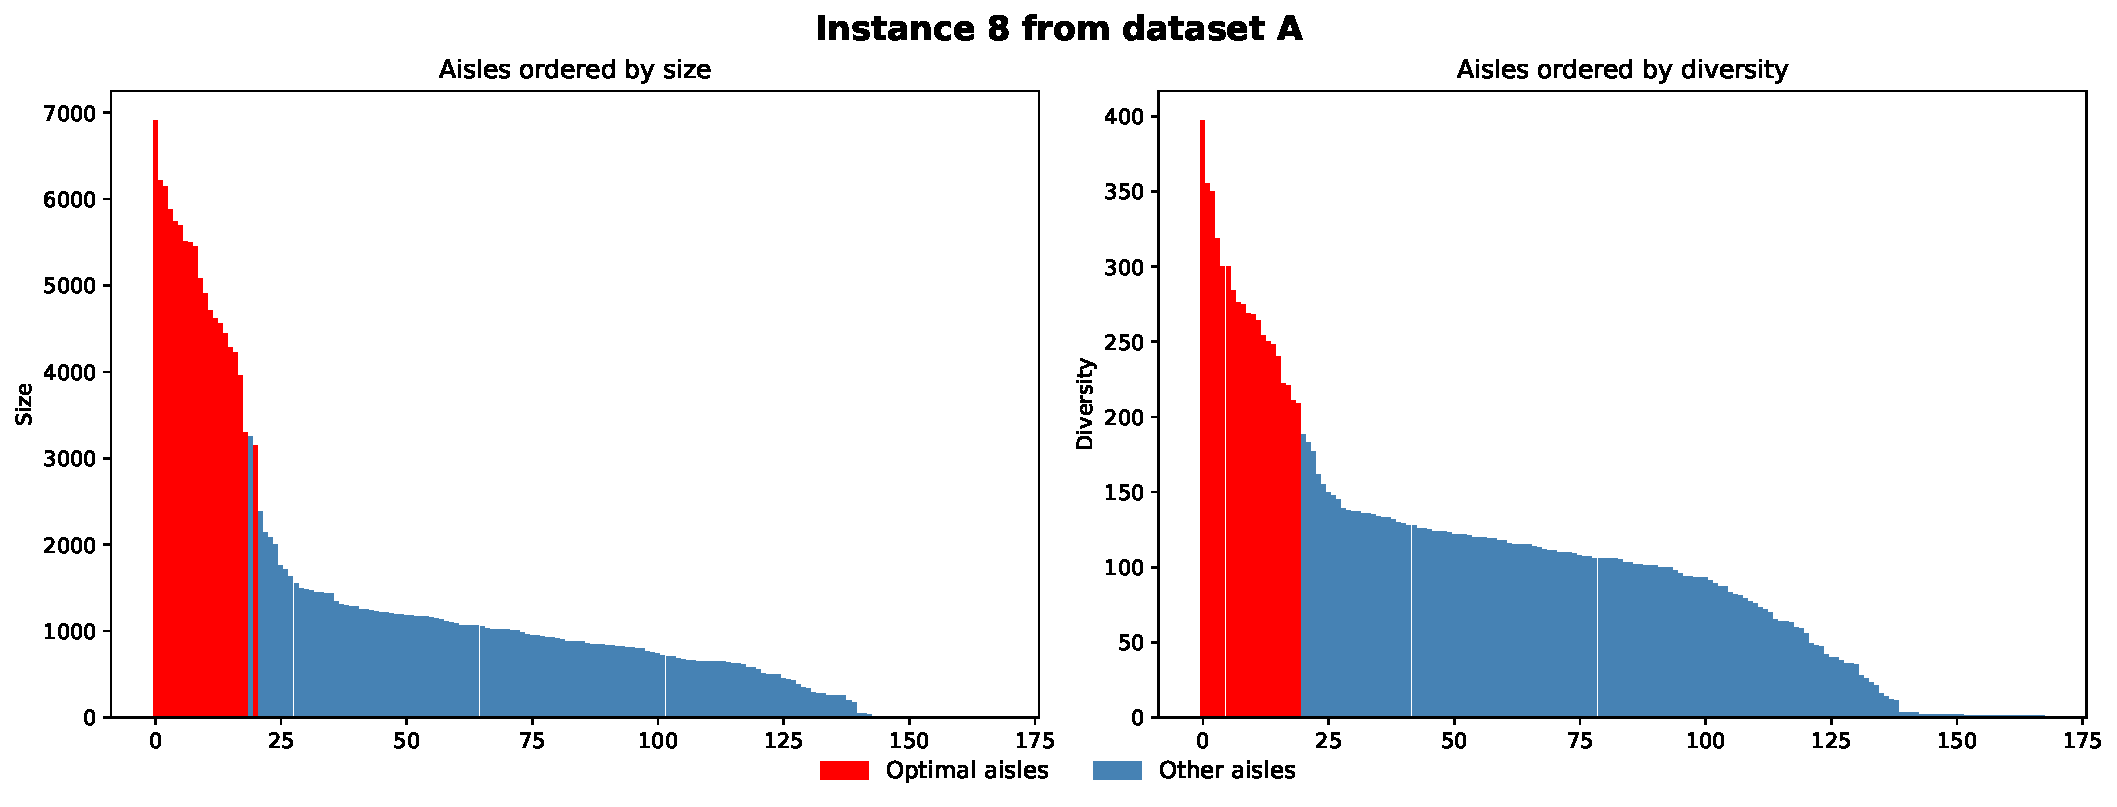
\includegraphics[width=0.8\textwidth]{greedy_instance_a.pdf}
      \caption{Aisles sorted by size and diversity and optimal aisles for instance 8 from dataset A.}
      \label{fig:aisles_greedy}
    \end{figure}

    \begin{columns}
  \begin{column}{0.45\textwidth}
  \justify
  Our algorithm fixes, for each possible $k$, the first $k$ aisles sorted based on each of these two criteria, and then picks orders greedily sorting them by size. Our implementation is efficient with complexity almost linear in the input size,
    and usually finds solutions 10\%-close to the optimal one in the order of seconds, as can be seen in Figure~\ref{fig:greedy_vs_optimal}. In most cases the greedy approach based on diversity beats the one based on size.
  \end{column}
  \begin{column}{0.55\textwidth}  %%<--- here
  \begin{center}
        \begin{figure}
        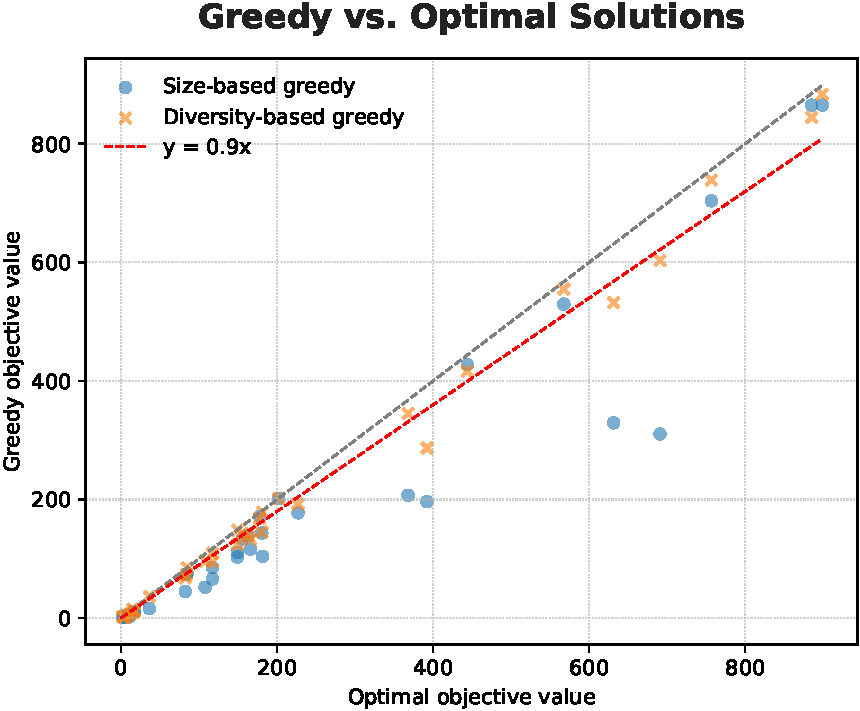
\includegraphics{greedy_vs_optimal.pdf}
        \caption{Comparison between the optimal values and the results given by the greedy algorithms.}
        \label{fig:greedy_vs_optimal}
      \end{figure}
    \end{center}
     \end{column}
  \end{columns}


    
  \end{block}

  \begin{block}{Local Search Iteration}

    Experimentally we see that after the first iterations of the Dinkelbach algorithm the aisles do not change that much. This motivates the idea of
    enforcing the condition that the next solution found must differ from the current one by at most $C$ aisles, which can be captured using the linear constraint
    
    \[
    \sum_{a \in A_i} y_a - \sum_{a \in A \setminus A_i} y_a \leq C
    \]

    where $A_i$ denotes the aisles from the solution at iteration $i$ and $y_a$ is the indicator variable for aisle $a$. If an iteration includes this constraint it is faster at the potential cost of optimality. Thus, in our final algorithm we alternate between local and non-local iterations.
  
  \end{block}

\end{column}

\separatorcolumn

\begin{column}{\colwidth}

  \begin{exampleblock}{A highlighted block containing some math}

    A different kind of highlighted block.

    $$
    \int_{-\infty}^{\infty} e^{-x^2}\,dx = \sqrt{\pi}
    $$

    Interdum et malesuada fames $\{1, 4, 9, \ldots\}$ ac ante ipsum primis in
    faucibus. Cras eleifend dolor eu nulla suscipit suscipit. Sed lobortis non
    felis id vulputate.

    \heading{A heading inside a block}

    Praesent consectetur mi $x^2 + y^2$ metus, nec vestibulum justo viverra
    nec. Proin eget nulla pretium, egestas magna aliquam, mollis neque. Vivamus
    dictum $\mathbf{u}^\intercal\mathbf{v}$ sagittis odio, vel porta erat
    congue sed. Maecenas ut dolor quis arcu auctor porttitor.

    \heading{Another heading inside a block}

    Sed augue erat, scelerisque a purus ultricies, placerat porttitor neque.
    Donec $P(y \mid x)$ fermentum consectetur $\nabla_x P(y \mid x)$ sapien
    sagittis egestas. Duis eget leo euismod nunc viverra imperdiet nec id
    justo.

  \end{exampleblock}

  \begin{block}{Nullam vel erat at velit convallis laoreet}

    Class aptent taciti sociosqu ad litora torquent per conubia nostra, per
    inceptos himenaeos. Phasellus libero enim, gravida sed erat sit amet,
    scelerisque congue diam. Fusce dapibus dui ut augue pulvinar iaculis.

    \begin{table}
      \centering
      \begin{tabular}{l r r c}
        \toprule
        \textbf{First column} & \textbf{Second column} & \textbf{Third column} & \textbf{Fourth} \\
        \midrule
        Foo & 13.37 & 384,394 & $\alpha$ \\
        Bar & 2.17 & 1,392 & $\beta$ \\
        Baz & 3.14 & 83,742 & $\delta$ \\
        Qux & 7.59 & 974 & $\gamma$ \\
        \bottomrule
      \end{tabular}
      \caption{A table caption.}
    \end{table}

    Donec quis posuere ligula. Nunc feugiat elit a mi malesuada consequat. Sed
    imperdiet augue ac nibh aliquet tristique. Aenean eu tortor vulputate,
    eleifend lorem in, dictum urna. Proin auctor ante in augue tincidunt
    tempor. Proin pellentesque vulputate odio, ac gravida nulla posuere
    efficitur. Aenean at velit vel dolor blandit molestie. Mauris laoreet
    commodo quam, non luctus nibh ullamcorper in. Class aptent taciti sociosqu
    ad litora torquent per conubia nostra, per inceptos himenaeos.

    Nulla varius finibus volutpat. Mauris molestie lorem tincidunt, iaculis
    libero at, gravida ante. Phasellus at felis eu neque suscipit suscipit.
    Integer ullamcorper, dui nec pretium ornare, urna dolor consequat libero,
    in feugiat elit lorem euismod lacus. Pellentesque sit amet dolor mollis,
    auctor urna non, tempus sem.

  \end{block}

  \begin{block}{References}

    \nocite{*}
    \footnotesize{\bibliographystyle{plainnat}\bibliography{poster}}

  \end{block}

\end{column}

\separatorcolumn
\end{columns}
\end{frame}

\end{document}
